\section{評価}
本章では、提案システムの性能評価について述べる。本評価ではボランティアコンピューティングを活用したクラウドゲーミングシステムの実現可能性を評価することを目的とする。また、提案システムが実現可能であるときそれが有用な条件は、プレイヤーPCからデータセンターよりもボランティアの提供する遊休コンピュータに接続する方がネットワーク遅延が小さい状況である。提案システムの実現可能性を評価するため、通信性能の評価および、ゲームプレイにおけるQoEを測定するためにフレームレートの評価も行う。

まず、評価を行う環境について述べる。次に、クラウドゲームサーバ/クライアント間の通信性能の評価について述べる。その後、ゲームプレイ時のフレームレートの評価について述べる。最後に評価についての考察を述べる。

\subsection{評価環境}
既存のクラウドゲーミングシステムはクラウドのデータセンター上でクラウドゲームサーバが動作している。これに対し、提案システムはボランティアが提供する遊休コンピュータ上でクラウドゲームサーバを動作させることで、プレイヤーからデータセンターまでの遅延を削減することを目指した。一般にユーザコンピュータからデータセンターへの遅延は大きくても50ms程度であるが、提案システムでのゲームプレイ中に発生する遅延がこの基準を下回るかどうかを評価する。また、提案システムの通信を実現するために組み込んだトンネリングのオーバヘッドについても評価を行う。

評価を行う環境を図\ref{fig:expenv}のように構築した。ボランティアクラウドゲーミングコントローラは用意せず、クラウドサーバ上にはEdgeVPNのリンクを確立するために必要なXMPPサーバのみを用意した。プレイヤーPCの役割を果たすプレイヤーPCではgRPCクライアントとGamingAnywhereクライアントが動作する。また、遊休コンピュータの役割を果たす遊休コンピュータではgRPCサーバ、GamingAnywhereサーバおよびゲームが動作する。

\begin{figure*}[t]
    \centering
    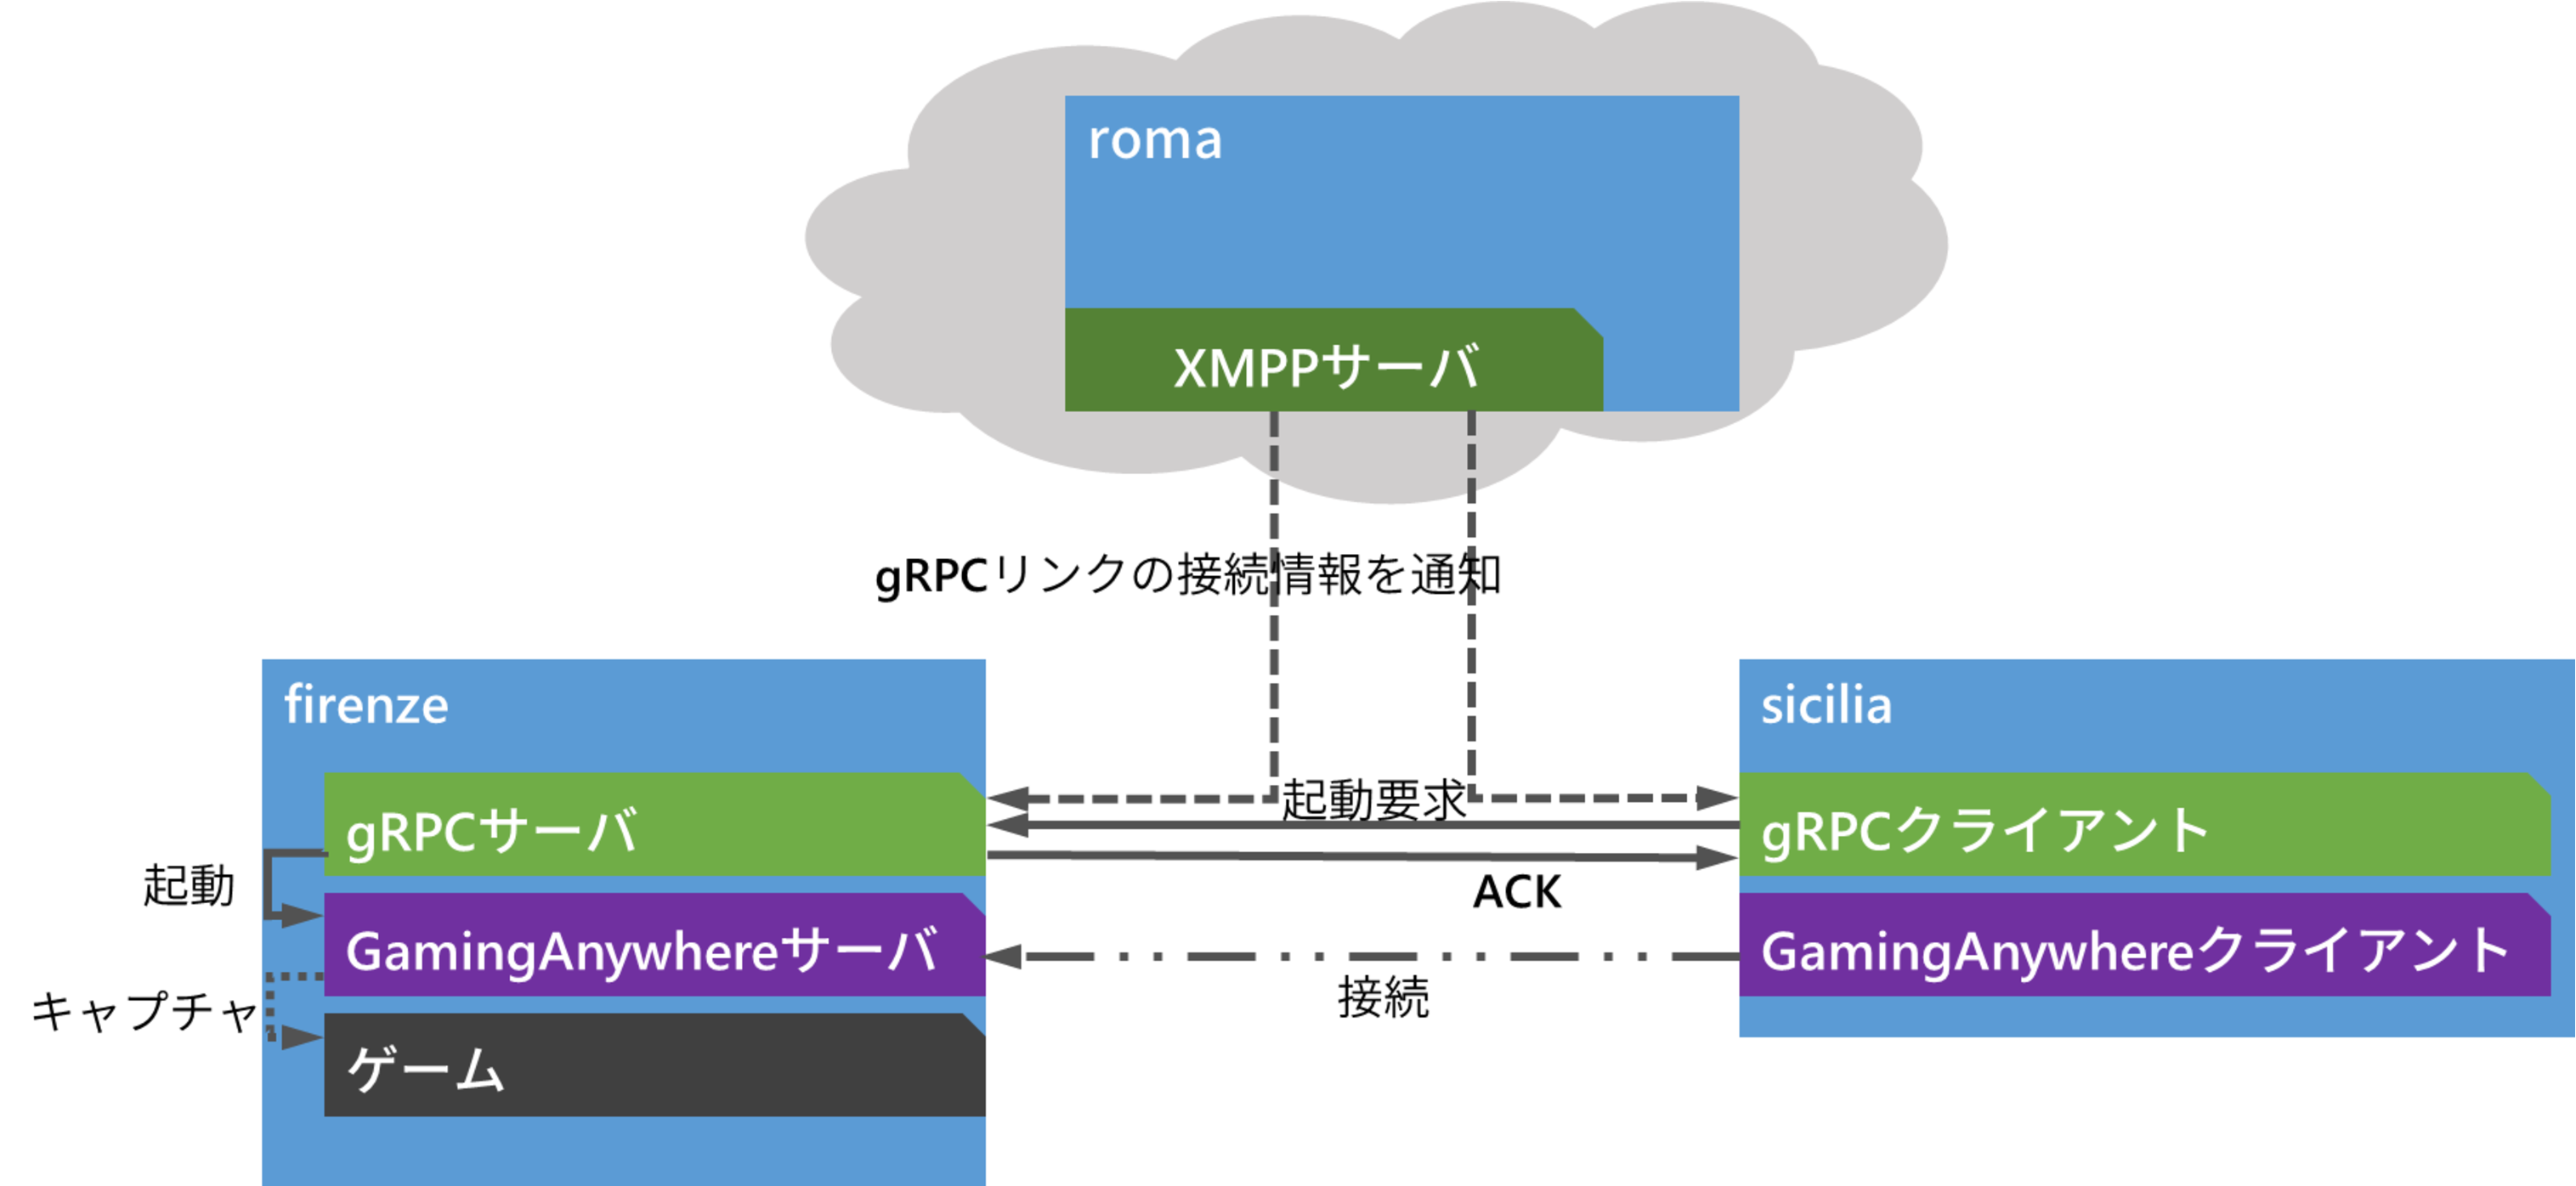
\includegraphics[width=0.8\textwidth,keepaspectratio,clip]{img/experimentalenvironment.eps}
    \caption{評価環境}
    \label{fig:expenv}
\end{figure*}

プレイヤーPCと遊休コンピュータはそれぞれUbuntu20.04で動作するマシンを用い、1Gbpsのリンクを持つネットワークで接続した。それぞれのマシンに2つのネットワークインターフェースを用意した。一つは管理用に使用し、もう一方はクラウドゲーミングのゲームデータの通信に使用している。ゲームデータ通信用のインターフェースに遅延の挿入や帯域制限をかけることにより、様々な環境のネットワークを再現して評価を行う。図\ref{fig:nic}のように、EdgeVPNを起動するとdockerコンテナが立ち上がり、それによってゲームデータ通信用のインターフェース上に仮想ネットワークインターフェースが立ち上がる。そこに仮想的なIPアドレスが割り当てられ、この仮想アドレスを持つインターフェースのペアでEdgeVPNのリンクが確立する。

EdgeVPNを利用しない条件で行う測定については、物理的なネットワークインターフェースに割り当てられているIPアドレスを用いてクラウドゲームサーバ/クライアントの接続を行い、直接通信をさせる。EdgeVPNを利用する条件での測定は、EdgeVPNによって生成された仮想ネットワークインターフェースに割り当てられている仮想IPアドレスを用いて通信を行うことで、VPN上における性能を測定する。

\begin{figure*}[t]
    \centering
    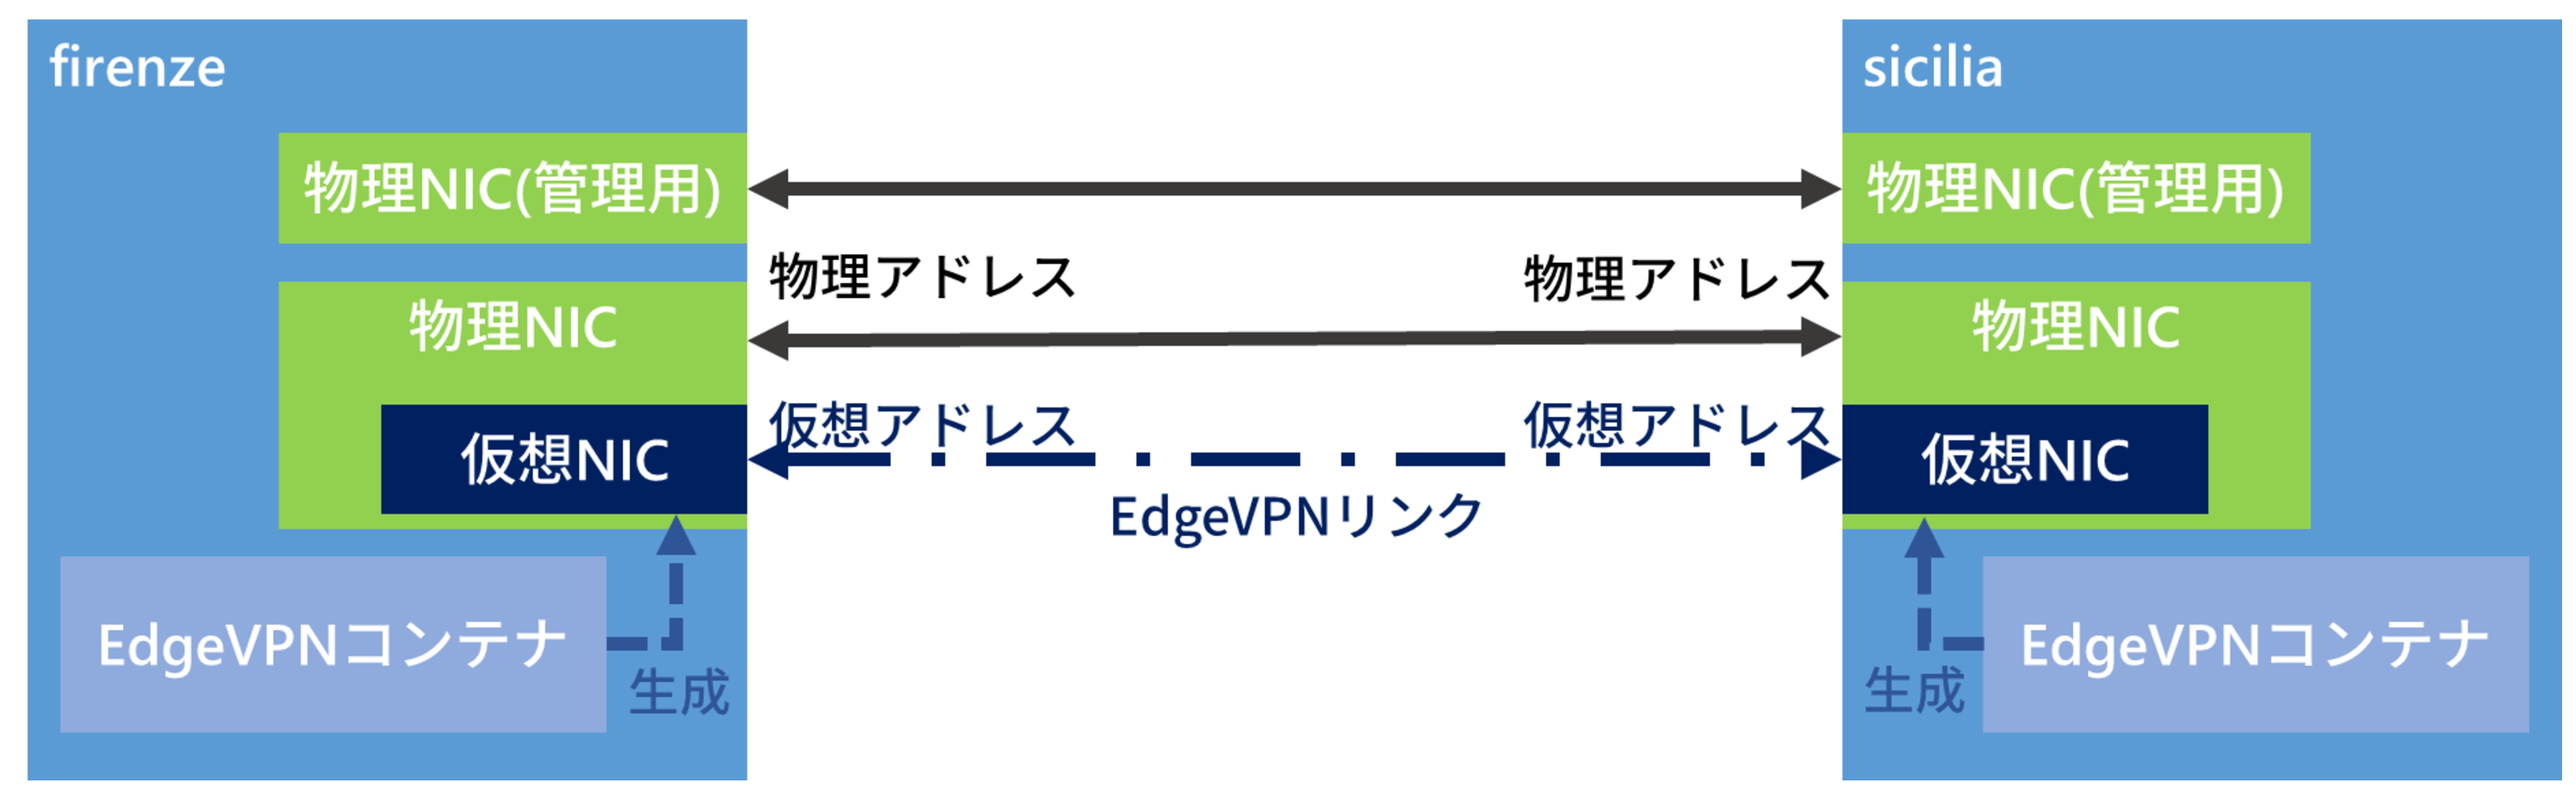
\includegraphics[width=0.8\textwidth,keepaspectratio,clip]{img/nic.eps}
    \caption{評価環境における通信}
    \label{fig:nic}
\end{figure*}

\subsection{クラウドゲームサーバ/クライアント間の通信性能}

\subsubsection{リンクに対する生の遅延の大小の影響}
プレイヤーPCと遊休コンピュータの間のネットワーク遅延の大小によって、GamingAnywhereサーバ/クライアント間のリンクを張るために使用しているEdgeVPNのオーバーヘッドがリンクの遅延に与える影響について調査した。tc\cite{iproute2}を用いてリンクに0-60msの遅延を挿入し、EdgeVPNを利用する場合と直接接続する場合の遅延増加の様子ping\cite{ping}を用いて計測した。遅延を挿入する際にコマンド\ref{add_ratency}のようにした。計測遅延と挿入遅延の値の差をプロットしたものが図\ref{fig:ratency}である。計測値にはpingを10回実行した際の値の平均値を使用している。

直接通信に比べて、EdgeVPNを利用する場合は平均して1ms程度遅延のオーバヘッドが存在することがわかる。また、遅延のオーバーヘッドは挿入遅延の大きさに関わらずほぼ一定であるといえる。

\begin{figure*}[t]
    \centering
    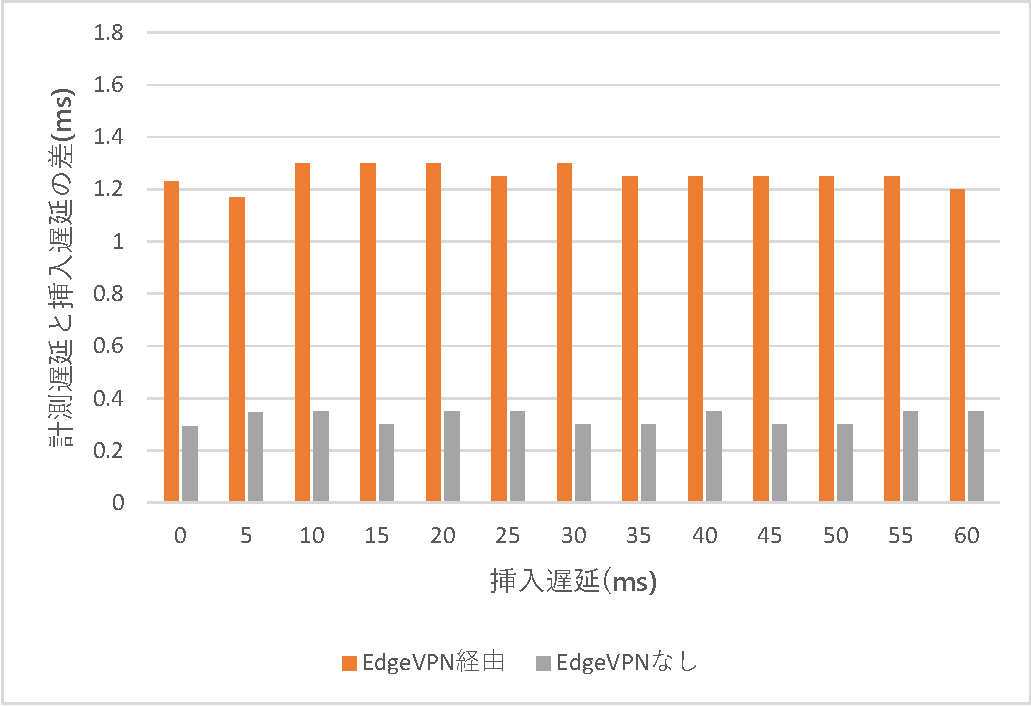
\includegraphics[width=0.8\textwidth,keepaspectratio,clip]{img/graph_ratency.pdf}
    \caption{EdgeVPNリンクに対する遅延挿入の影響}
    \label{fig:ratency}
\end{figure*}

\begin{lstlisting}[caption=遅延挿入,label=add_ratency]
    tc qdisc add dev brl101000F root netem delay 10ms
\end{lstlisting}

\subsubsection{リンクに対する遅延の大小のスループットへの影響}
プレイヤーPCと遊休コンピュータの間のネットワーク遅延の大小の影響で、GamingAnywhereサーバ/クライアント間のリンクで展開したEdgeVPNがリンクのネットワークスループットに与える影響について調査した。5.2.1と同様にtcを用いてリンクに0-60msの遅延を挿入し、EdgeVPNを利用する場合と直接接続する場合のスループット減少の様子をiperf\cite{iperf}を使用して計測した。計測値はiperfを60秒間の設定で10回実行した結果を用いている。EdgeVPNを利用する通信についての結果をプロットしたものが図\ref{fig:band_with_edge}、直接接続する通信についての結果をプロットしたものが図\ref{fig:band_without_edge}である。

EdgeVPNを利用する通信において、スループットが指数関数的に減少していることがわかる。一方で、最も大きい60msまで遅延が増大した状況下においても40Mbps程度のスループットをGamingAnywhereサーバ/クライアント間のリンクにおいて維持できている。

\begin{figure*}[t]
    \centering
    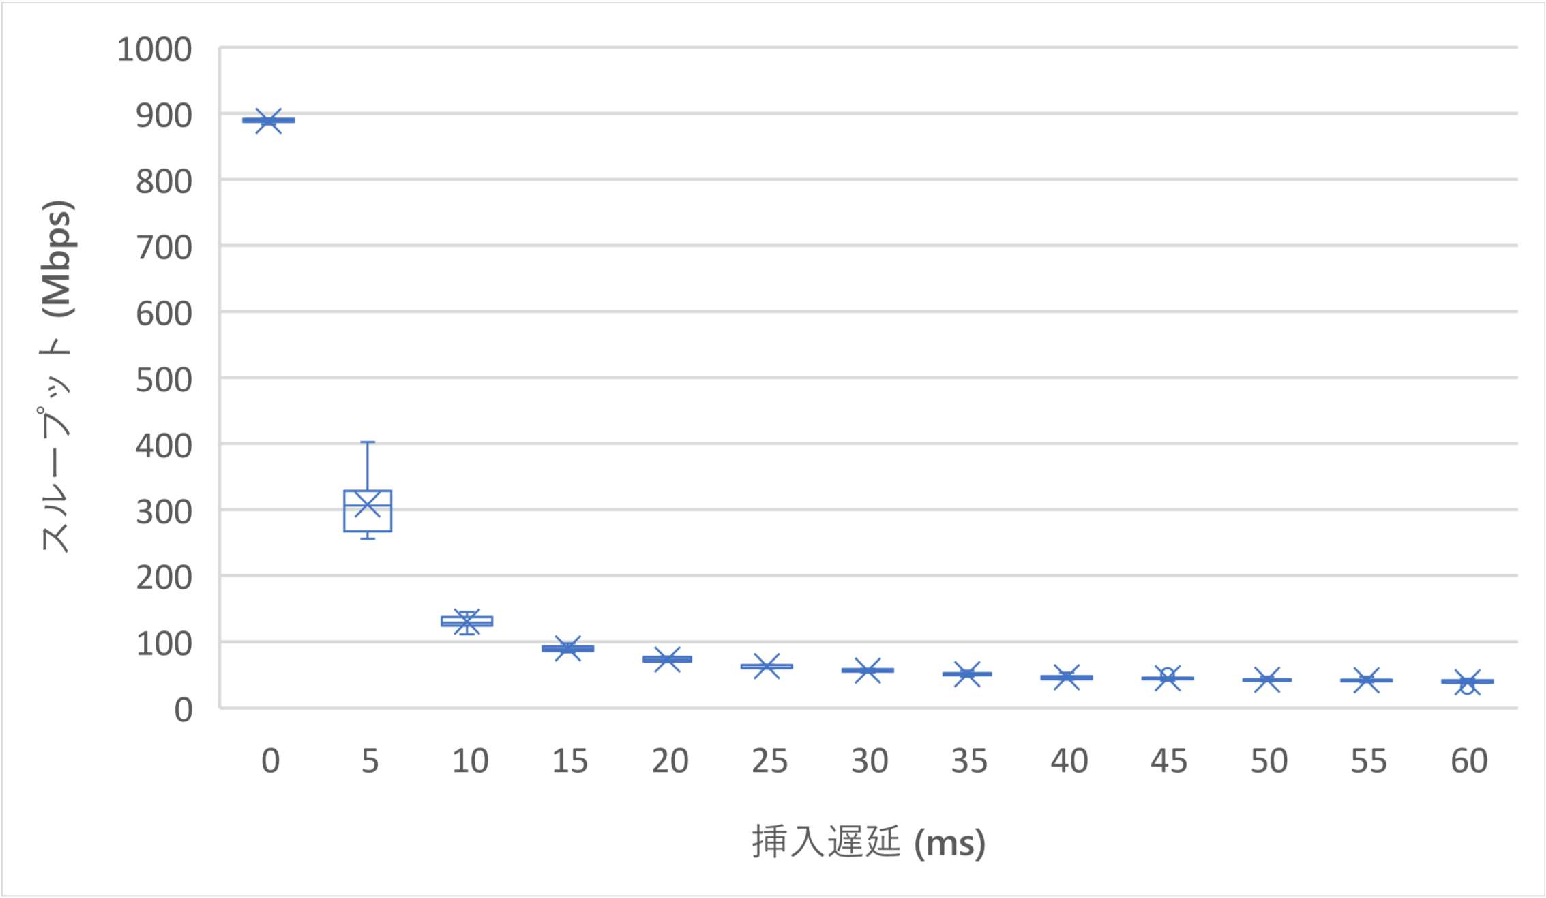
\includegraphics[width=0.8\textwidth,keepaspectratio,clip]{img/bandwidth_withEdgeVPN.pdf}
    \caption{EdgeVPNリンクへの遅延挿入の帯域への影響}
    \label{fig:band_with_edge}
\end{figure*}

\begin{figure*}[t]
    \centering
    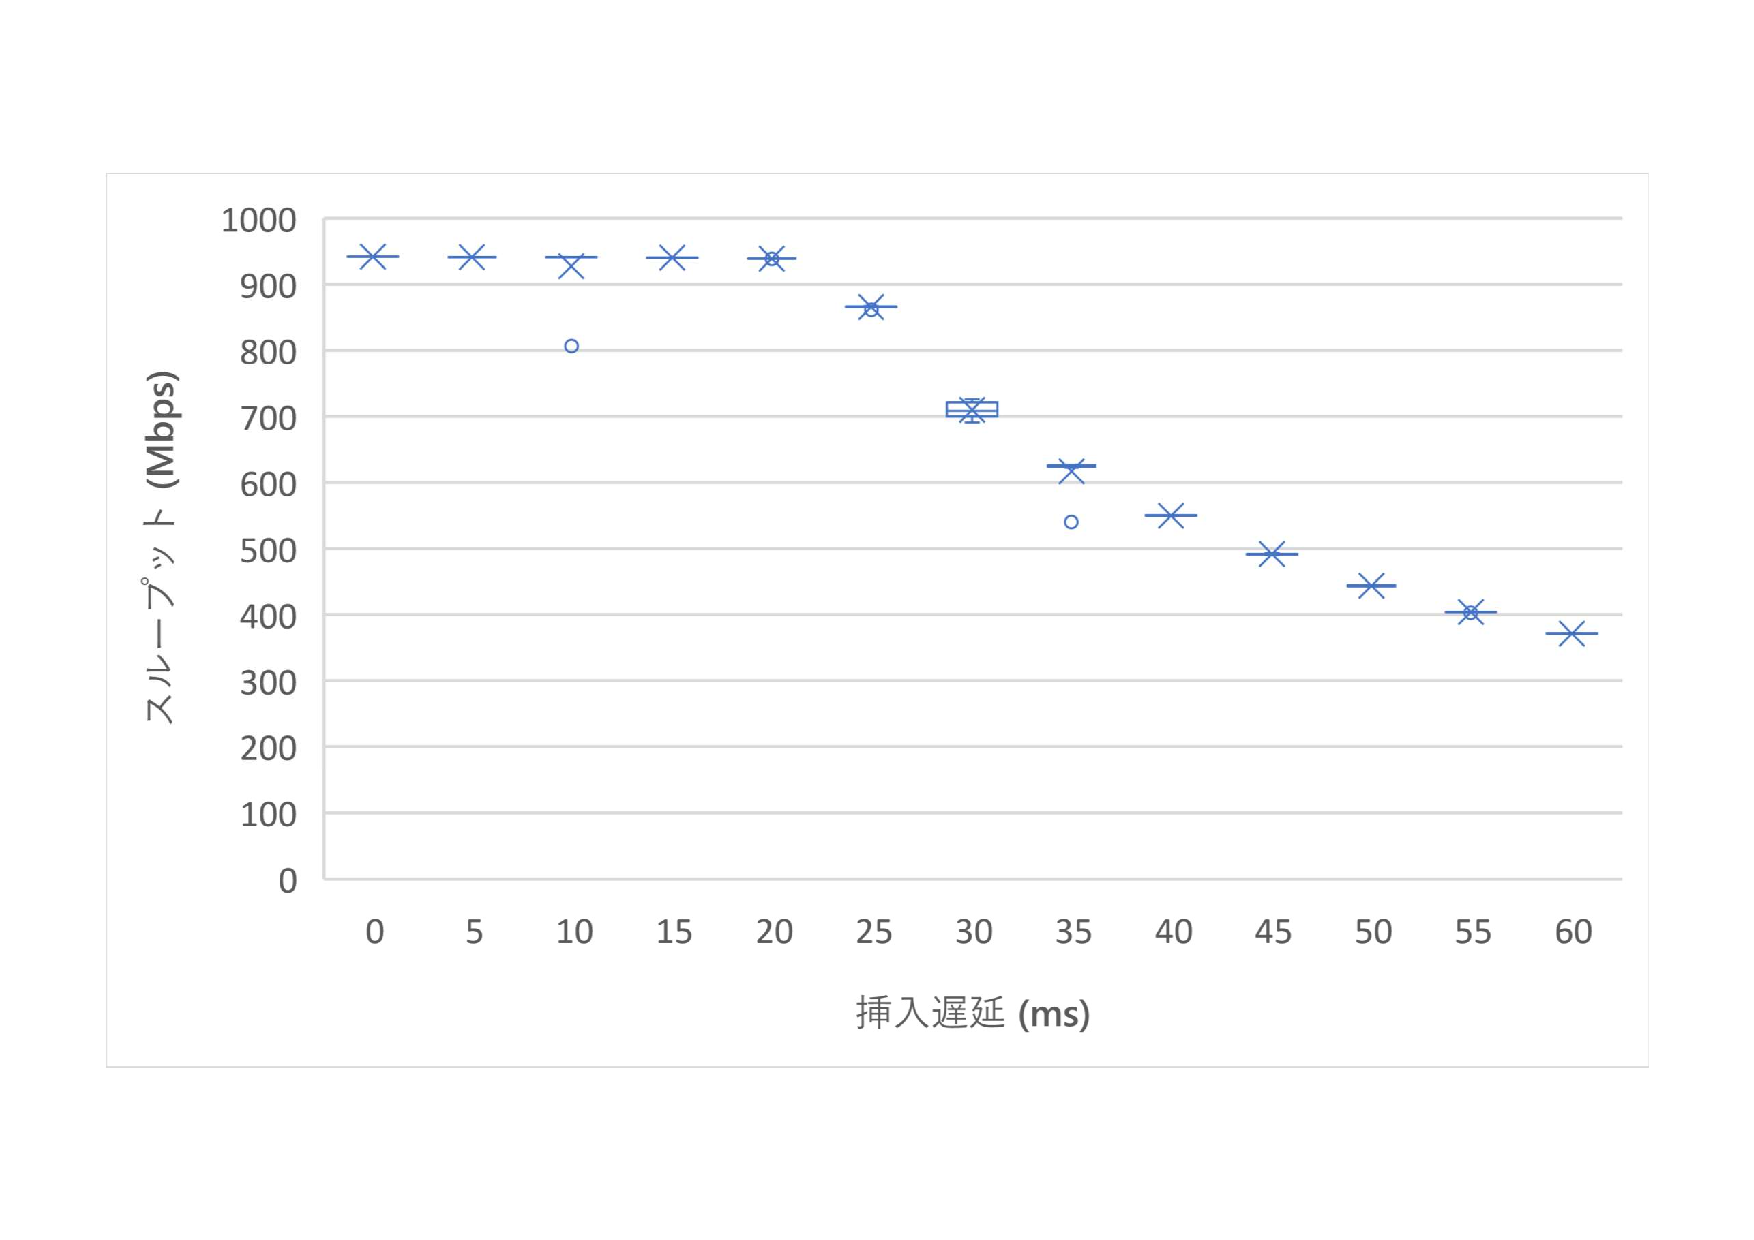
\includegraphics[width=0.8\textwidth,keepaspectratio,clip]{img/bandwidth_withoutEdgeVPN.pdf}
    \caption{EdgeVPNを使用していないリンクへの遅延挿入の帯域への影響}
    \label{fig:band_without_edge}
\end{figure*}

\subsubsection{10GbpsネットワークにおけるEdgeVPNのオーバーヘッド}
ネットワークインターフェースが1Gbpsの環境では、スループットの上限が1Gbpsに制限されているので、挿入遅延が0msの場合にEdgeVPNのオーバーヘッドの影響が分かりづらい (図\ref{fig:band_with_edge}、\ref{fig:band_without_edge}) 。この結果はEdgeVPNによる性能低下を正確に測定できていない可能性がある。

そこで、仮想環境にはなるが10Gbpsネットワークが利用可能な環境における実験を行った。異なる物理マシンで動作する10Gbpsで接続された2つのVMを用意し、EdgeVPNでリンクを張るインターフェースと直接接続をするインターフェースをそれぞれ用意した。5.2.2節と同様に遅延挿入を行ってスループット減少の様子を観測した。EdgeVPNを利用する通信についての結果は図\ref{fig:band_withedge_vm}、直接接続する通信についての結果は図\ref{fig:band_withoutedge_vm}である。10GbpsネットワークにおいてはEdgeVPNを利用すると、遅延挿入を行っていなくても550Mbps程度までスループットが下がっていることがわかる。この値が1Gbpsネットワークでの結果よりも低いのは、VMのオーバヘッドによるものと考えられる。また、遅延挿入に伴ってばらつきはあるもののスループットの減少が見られ、60msのネットワーク遅延がある状態では最低で35Mbps程度まで低下している。オーバーヘッドは大きいものの、10Gbps環境においてもクラウドゲーミングのプレイに耐える程度の性能を発揮していると言える。

%\begin{figure*}[t]
%    \centering
%    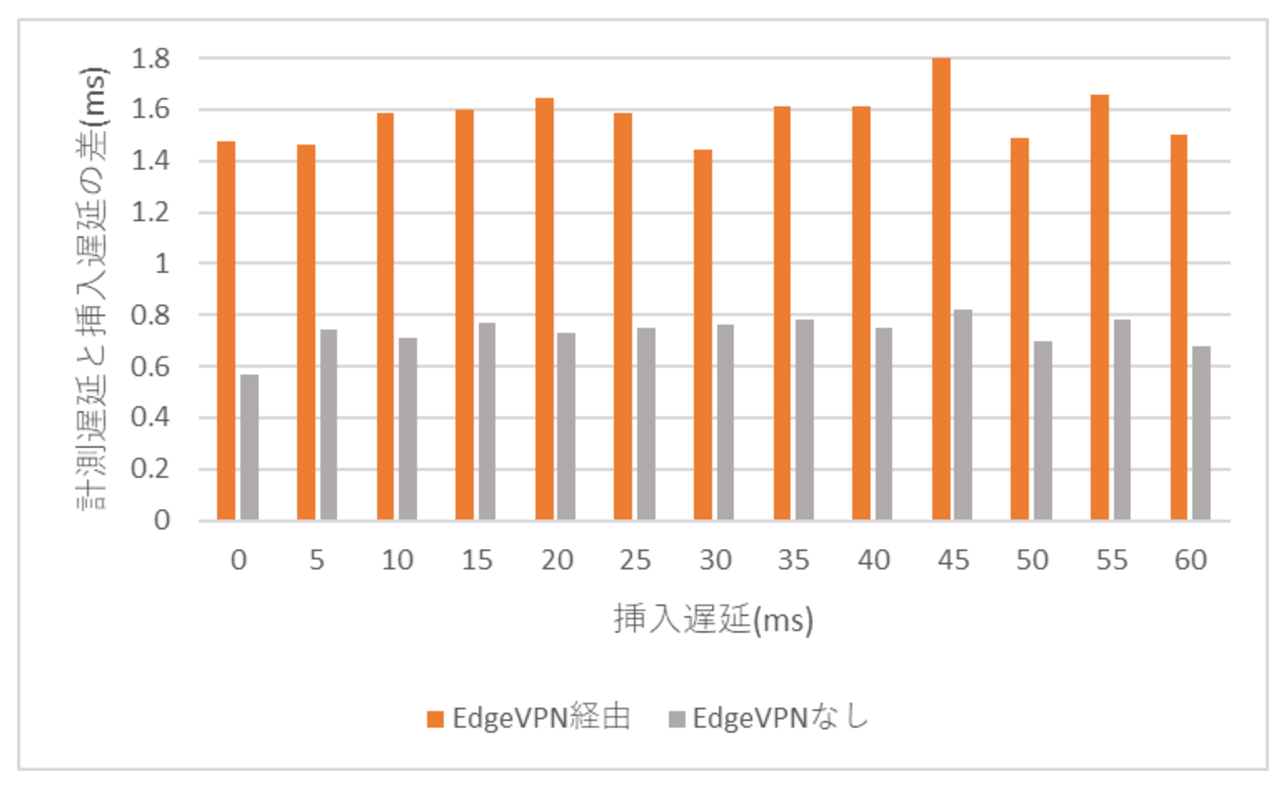
\includegraphics[width=0.8\textwidth,keepaspectratio,clip]{img/ratency_vm.eps}
%    \caption{10GbpsネットワークにおけるEdgeVPNリンクに対する遅延挿入の影響}
%   \label{fig:ratency_vm}
%\end{figure*}

\begin{figure*}[t]
    \centering
    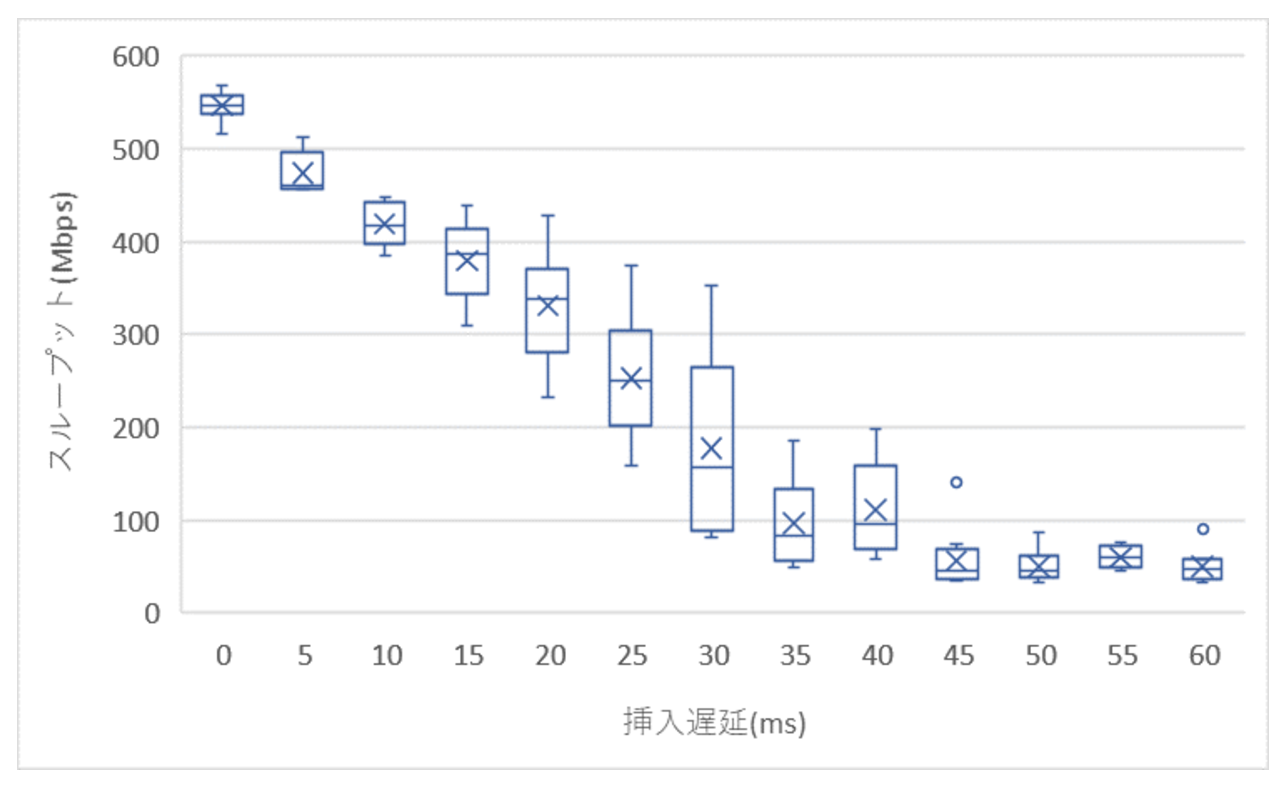
\includegraphics[width=0.8\textwidth,keepaspectratio,clip]{img/band_withedge_vm.eps}
    \caption{10GbpsネットワークにおけるEdgeVPNリンクへの遅延挿入の帯域への影響}
    \label{fig:band_withedge_vm}
\end{figure*}

\begin{figure*}[t]
    \centering
    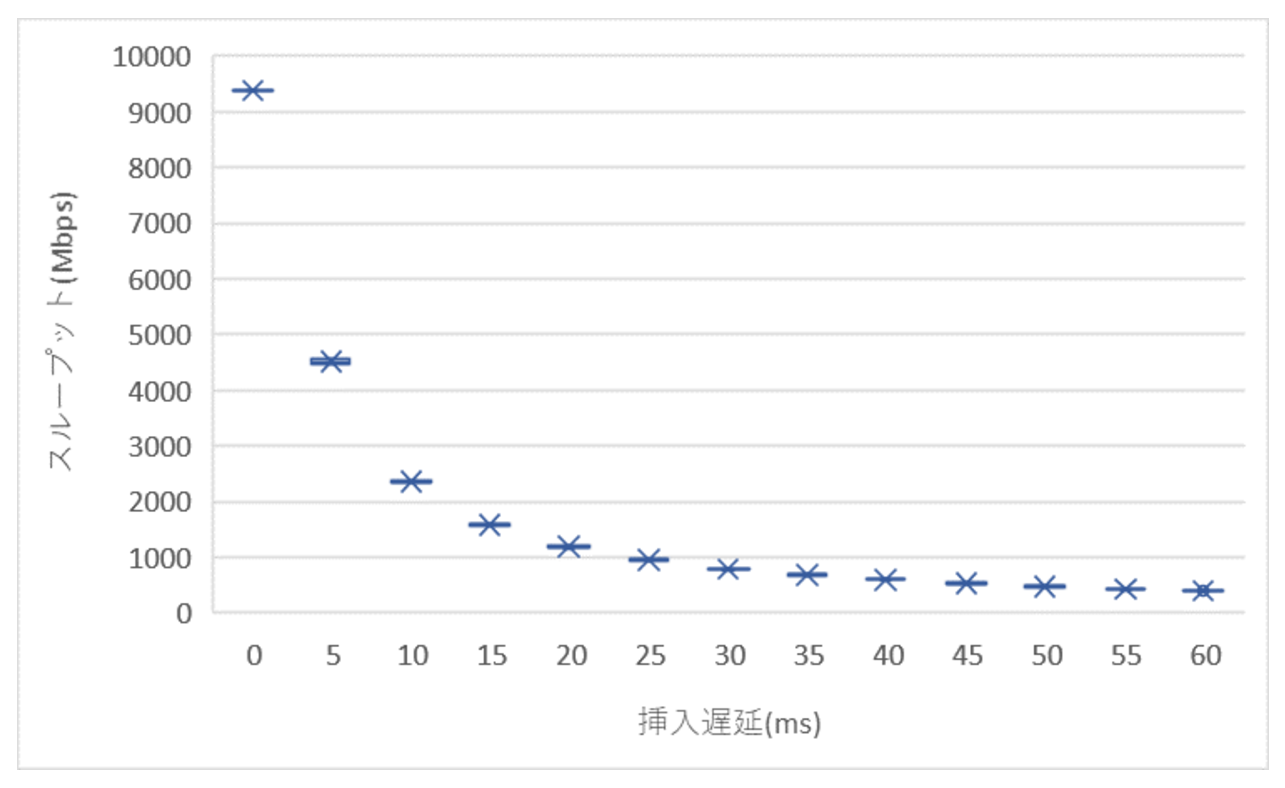
\includegraphics[width=0.8\textwidth,keepaspectratio,clip]{img/band_withoutedge_vm.eps}
    \caption{10GbpsネットワークにおけるEdgeVPNを使用していないリンクへの遅延挿入の帯域への影響}
    \label{fig:band_withoutedge_vm}
\end{figure*}

\subsection{ゲームプレイ時のフレームレート}

\subsubsection{ネットワーク帯域の大小の影響}
提案システムを使用して実際にゲームをプレイしている間、プレイヤーPCと遊休コンピュータの間のネットワーク帯域幅のサイズがゲーム画面のフレームレートにどのように影響するかを調査した。

実験はGamingAnywhereサーバの設定でフレームレートを60fpsに設定した状態で行った。ゲームのジャンルにより画面の動きが激しく、フレームレートの変動の影響が大きいものとそうでないものがあるため、複数のジャンルから選んだゲームを実験に使用した。実験に使用したゲームはMMORPGに分類されるAlbion Online\cite{albiononline}、FPS/アクションに分類されるRed Eclipse 2\cite{redeclipse}、およびボードゲームであるSimply Chess\cite{simplychess}の3種類である。いずれもPCゲームのダウンロード販売等を行うプラットフォームであるSteam\cite{steam}で公開されている、Linuxに対応したゲームである。

\begin{figure*}[t]
    \centering
    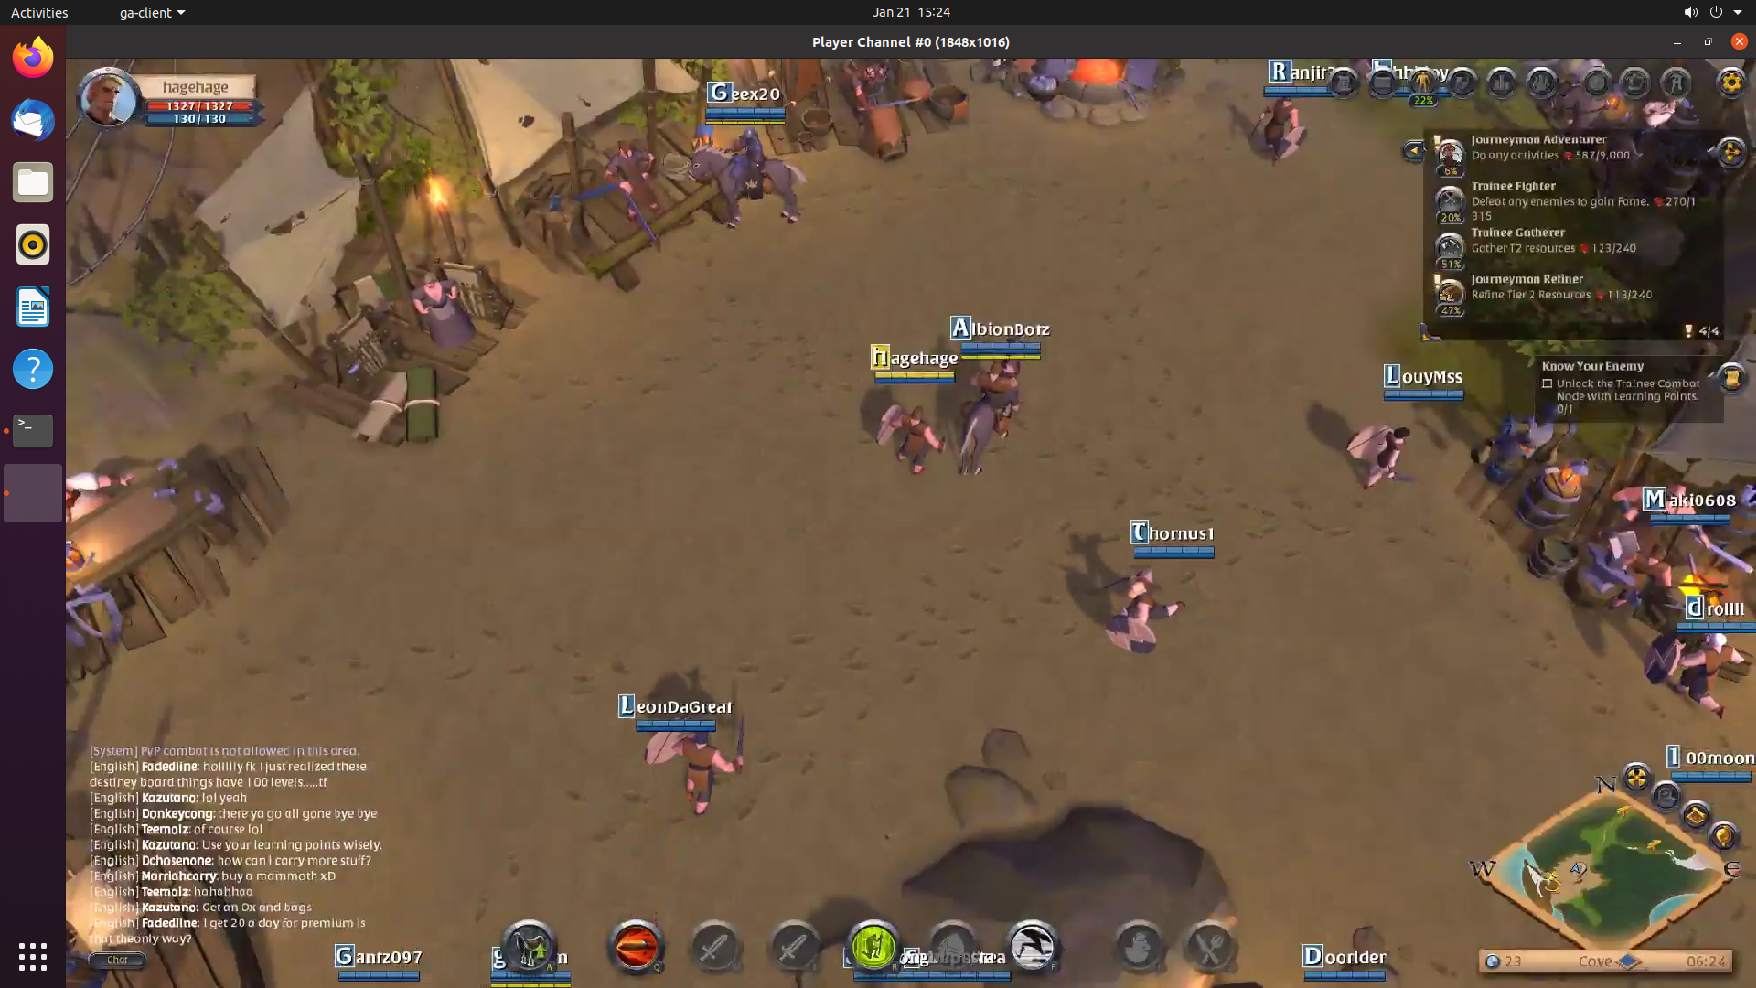
\includegraphics[width=0.8\textwidth,keepaspectratio,clip]{img/screen_mmo.pdf}
    \caption{提案システムを使用したAlbion Online (MMORPG)のプレイの様子}
    \label{fig:screen_mmo}
\end{figure*}

\begin{figure*}[t]
    \centering
    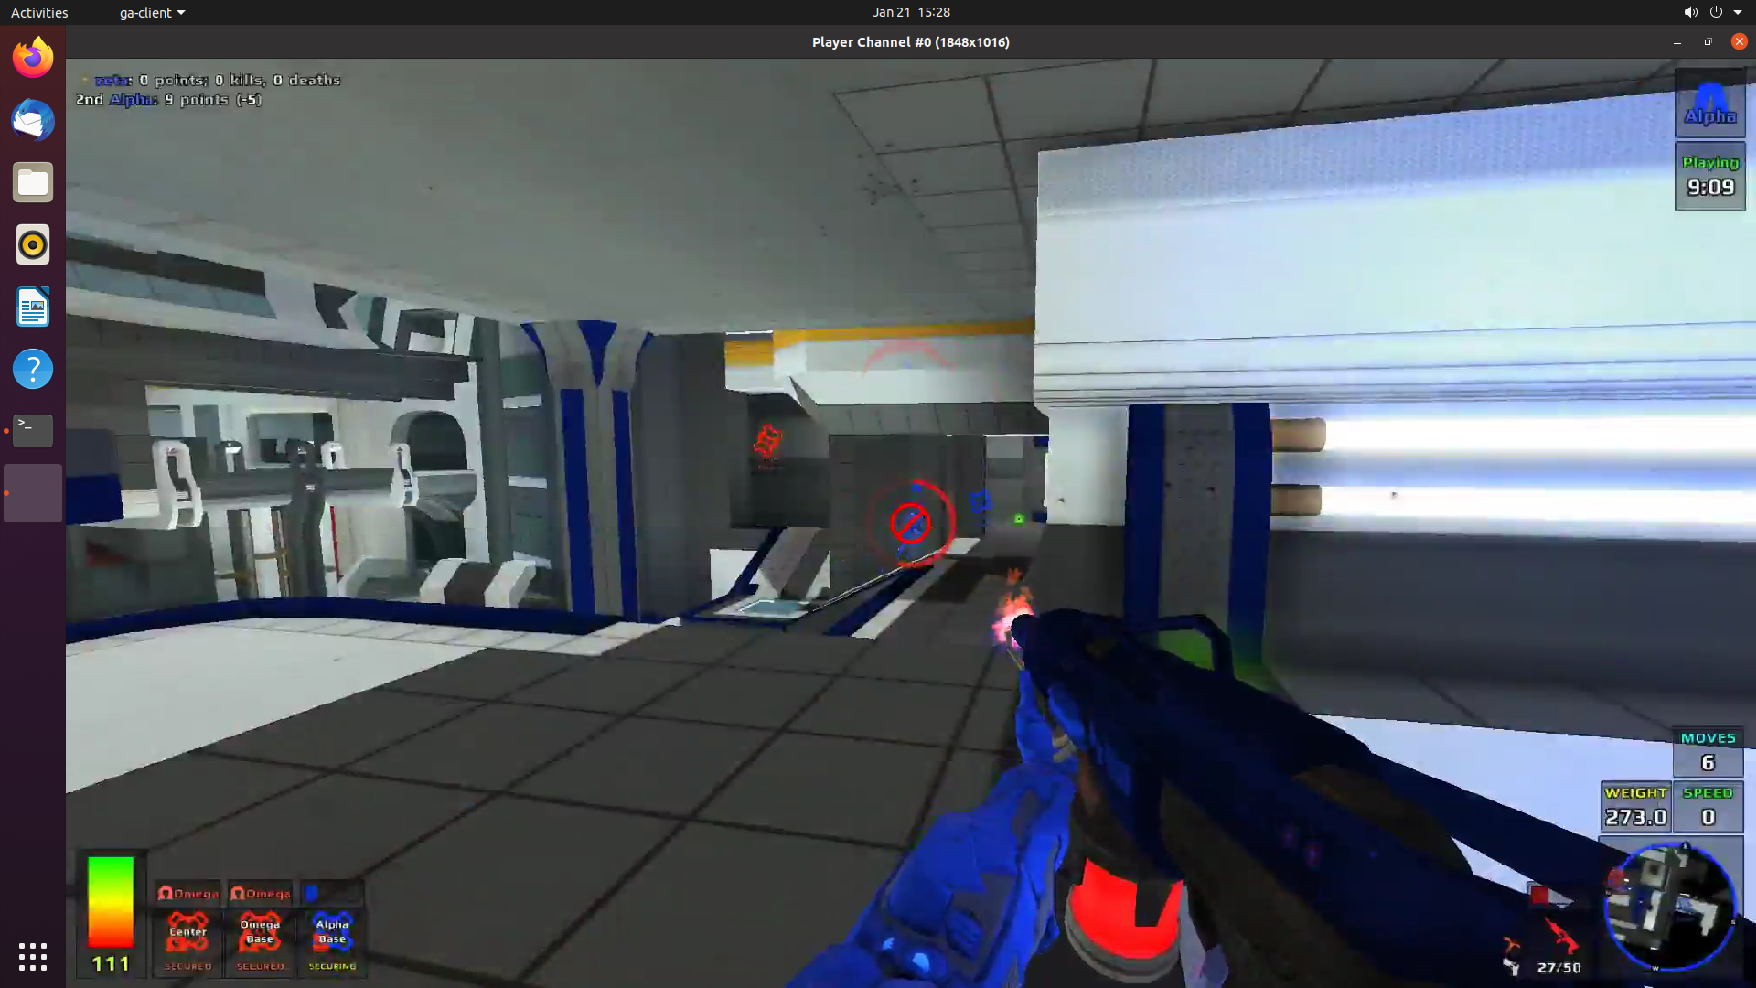
\includegraphics[width=0.8\textwidth,keepaspectratio,clip]{img/screen_fps.pdf}
    \caption{提案システムを使用したRed Ecliplse 2 (FPS, Action)のプレイの様子}
    \label{fig:screen_fps}
\end{figure*}

\begin{figure*}[t]
    \centering
    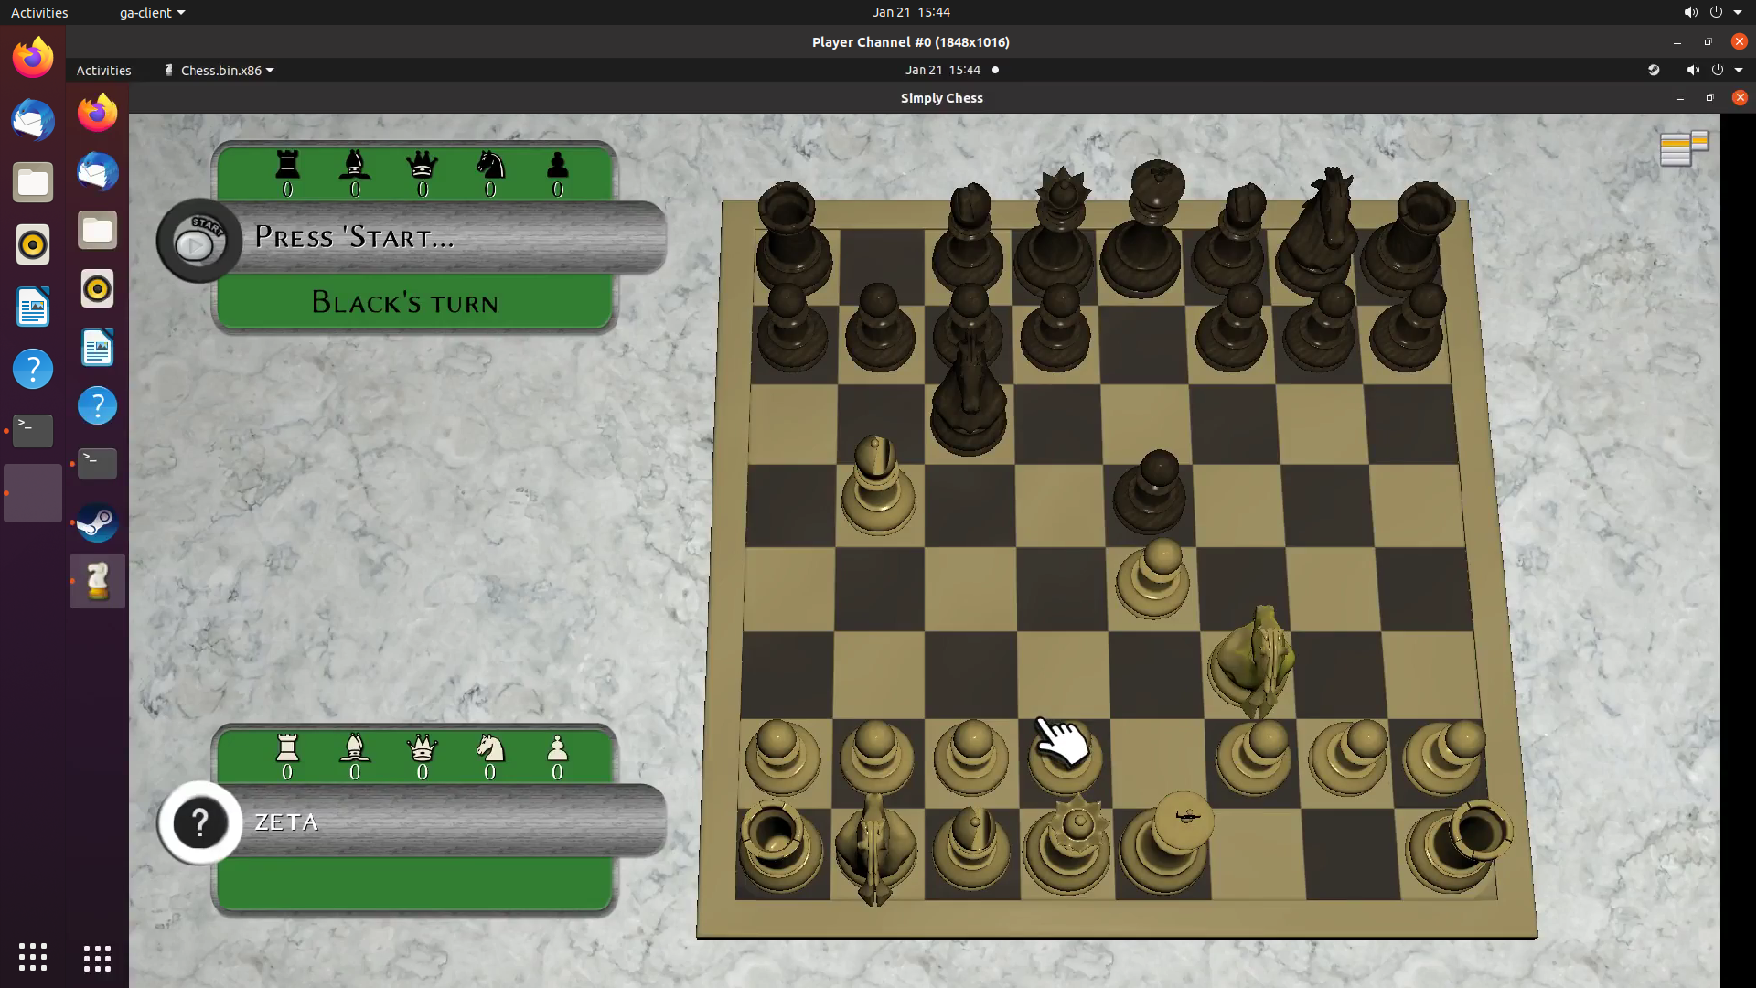
\includegraphics[width=0.8\textwidth,keepaspectratio,clip]{img/screen_board.pdf}
    \caption{提案システムを使用したSimply Chess (ボードゲーム)のプレイの様子}
    \label{fig:screen_board}
\end{figure*}

GamingAnywhereサーバ/クライアント間のリンクにtcを使用して帯域制限を施し、EdgeVPNを利用する場合と直接接続する場合のそれぞれについてフレームレートの変化を観測した。帯域制限は、制限をかけていない1Gbpsおよび100Mbpsと10Mbpsの3つの条件で行った。計測値はGamingAnywhereクライアントが定期的に出力するフレームレートの値を10回分計測し、その平均値を使用している。Albion Onlineをプレイした際の結果を図\ref{fig:fps_mmo}、Red Eclipse 2をプレイした際の結果を図\ref{fig:fps_fps}、Simply Chessをプレイした際の結果を図\ref{fig:fps_board}にそれぞれ示した。

動きのあまり少ないボードゲームのSimply Chessのプレイ中においてはEdgeVPNを利用するかどうかに関わらず、帯域制限下でもほぼ60fpsのフレームレートを保っている。また、常に画面の少なくとも一部に動きが生じるジャンルであるMMORPGのAlbion Onlineのプレイ中においても、帯域制限下で60fpsを大きく下回ることなくパフォーマンスが安定している。さらに、常に画面全体に激しい動きが発生するFPS/アクションに分類されるRed Eclipse 2のプレイ中においても、帯域制限下でフレームレートの低下は確認されなかった。

\begin{figure*}[t]
    \centering
    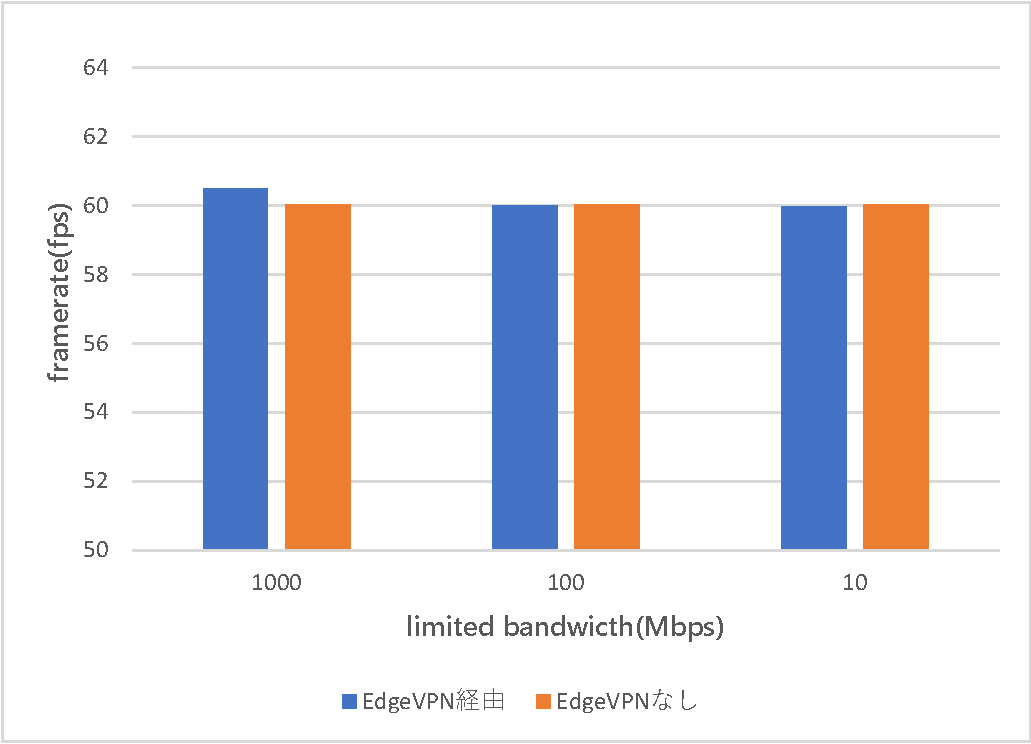
\includegraphics[width=0.8\textwidth,keepaspectratio,clip]{img/framerate_MMO.pdf}
    \caption{帯域制限下でのゲームプレイ時のフレームレートの変化 (Albion Online (MMORPG)プレイ時)}
    \label{fig:fps_mmo}
\end{figure*}

\begin{figure*}[t]
    \centering
    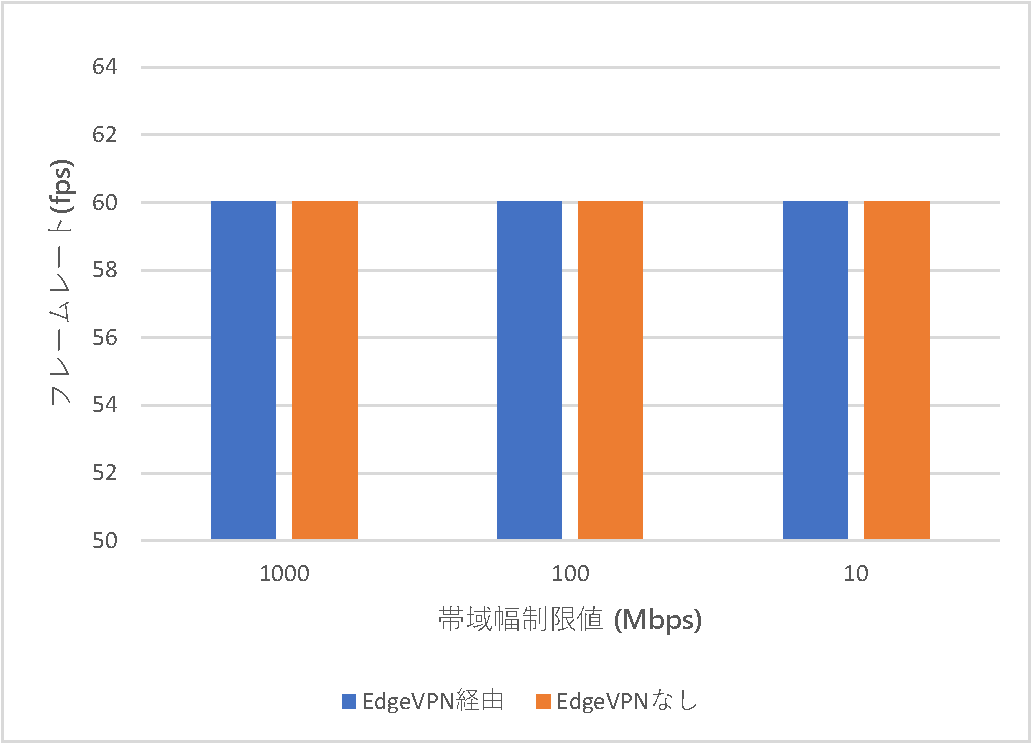
\includegraphics[width=0.8\textwidth,keepaspectratio,clip]{img/framerate_FPS.pdf}
    \caption{帯域制限下でのゲームプレイ時のフレームレートの変化 (Red Ecliplse 2 (FPS, Action)プレイ時)}
    \label{fig:fps_fps}
\end{figure*}

\begin{figure*}[t]
    \centering
    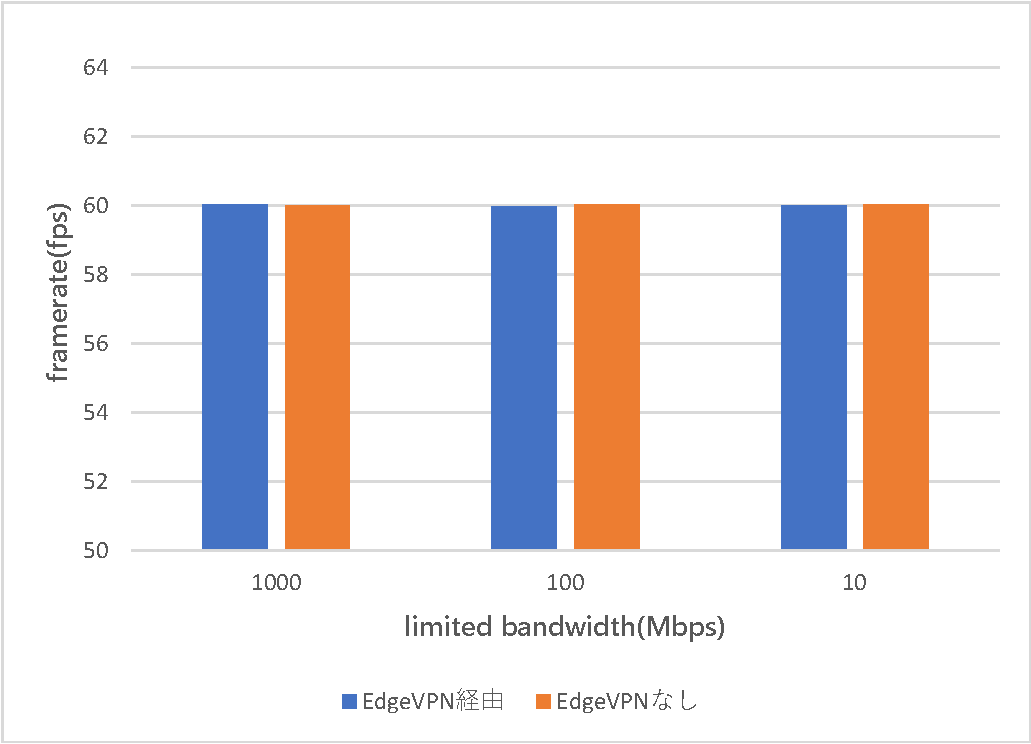
\includegraphics[width=0.8\textwidth,keepaspectratio,clip]{img/framerate_Board.pdf}
    \caption{帯域制限下でのゲームプレイ時のフレームレートの変化 (Simply Chess (ボードゲーム)プレイ時)}
    \label{fig:fps_board}
\end{figure*}

\subsection{考察}
国内のデータセンターにユーザコンピュータが接続する場合のネットワーク遅延は最大50ms程度である。提案システムにおいて、プレイヤーPCが接続するボランティアが提供する遊休コンピュータまでのネットワーク遅延がこれよりも小さい場合に、クラウドゲーミングのQoEを損なわないパフォーマンスを提供できるかどうかを考察する。

まず、クラウドゲーム/サーバ間のリンクのネットワーク遅延について、EdgeVPNのオーバーヘッドにより直接接続のネットワークよりも1ms程度遅延が増えている。この遅延の増大はゲームプレイに影響を及ぼす程度のものではなく許容量であるといえる。

また、リンクにEdgeVPNを使用したことにより、リンクのネットワーク遅延が大きくなるに伴ってスループットが低下する。計測値のうち最も低くなるリンクのネットワーク遅延が60msの場合のスループットは40Mbps程度である。Google Stadiaをプレイするのに必要なネットワーク要件として最低25Mbpsのスループットのネットワーク接続が必要であると言われている\cite{stadia_band}。またPlaystation Nowは公式サイトにて、快適にプレイするため必要なネットワーク要件として12Mbps以上のスループットを上げている\cite{ps-now}。提案システムはこれらの要件を満たしており、クラウドゲーミングのプレイに充分なスループットを維持できると言える。

さらに、EdgeVPNのオーバーヘッドがゲームプレイ時のフレームレートに与える影響について調べた。その結果、10Mbpsの低スループットのネットワークを使用した場合においてもフレームレートの低下は見られなかった。これは、ボードゲームのような画面の動きが小さいゲームのみならず、FPSのような常に激しい画面の動きを伴うゲームにおいても同様である。

以上より、提案システムはデータセンターよりもネットワーク遅延の小さい遊休コンピュータでクラウドサーバをホストした場合に、QoEを損なわないクラウドゲーミングのプレイに十分な性能を示した。



